\chapter{Prior and posterior analyses}

\section{Pre-treatment}

1D-3C SEM codes provides PRE and POST folders for simple prior and posterior analyses to simulations. First, in PRE directory, a Python script ‘create \textunderscore mesh.py’  is provided for mesh file creation which is required for the code to define the coordinates of element nodes and boundary conditions. \\

The script is self-explanatory and interactive. First, the user is asked to specify the name of the mesh file to be created and its explanation. Then, total element number, total domain number and upper boundary condition should be defined. Afterwards, the script needs the set of element sizes to be used. In Figure \ref{cremesh}, an example for a model of 20 meters depth which is composed of two elements is shown. Once element sizes are defined, for each domain of the model, the scripts asks total number of element for each element size. To finish, bottom boundary condition is necessary. \\



%% FIGURE : create_mesh.py
\begin{center}
\leavevmode
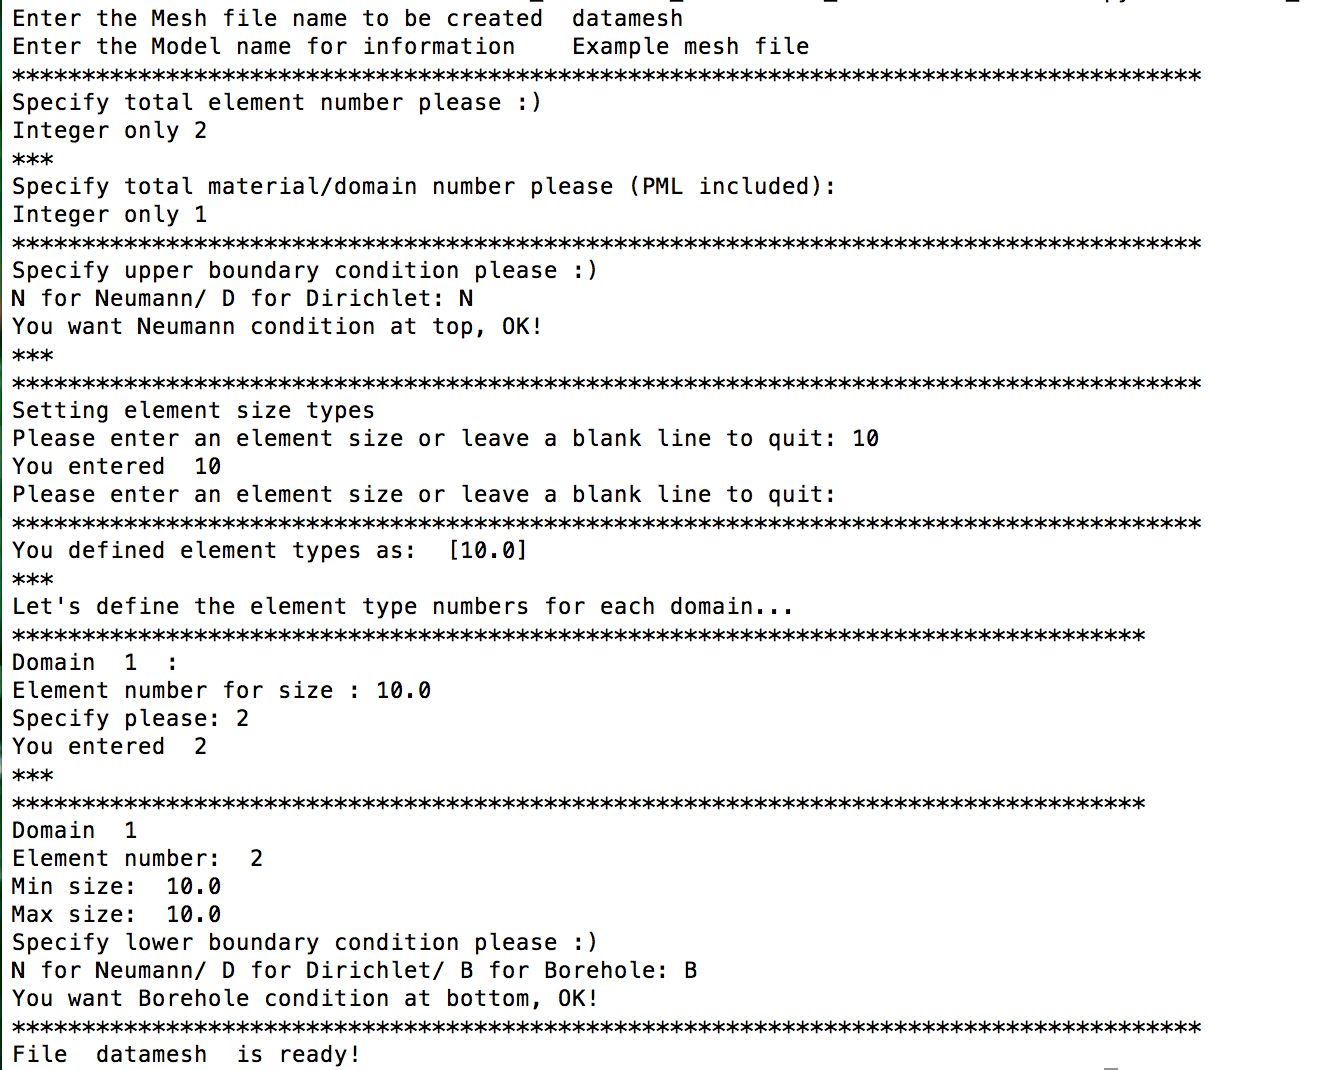
\includegraphics[scale=0.65]{figures/createmeshpy.eps} 
\captionof{figure}{create \textunderscore mesh.py file for 1D mesh file creation.}
\label{cremesh} 
\vspace{1cm}
\end{center}



\section{Post-treatment}

\label{sec:prepost}

Once the simulation terminates, the code sorts a number of output files. For all rheological models (elastic, viscoelastic, nonlinear cases), acceleration, velocity time histories in three directions of the first series of receivers are saved. Also, stress and strain parameters for the second series of receivers are written out in files. \\ 

For pressure-independent nonlinear models, such as P1 example, additionally a file with backbone curve strain and stress parameters is furnished. Depending on curve type (hyperbolic or experimental), the file name is named SOILHYPER or SOILEXP.  \\


For pressure-dependent models,  two additional files are provided. ‘PressSoilParams00X.dat’ file (where X refers to receiver number) includes shear modulus, Young modulus, bulk modulus, Poisson ratio, initial shear modulus after normalization and current maximum shear modulus, for each time step. In ‘PressEffectiveParams00X.dat’, current values of principal deviatoric stress, $W_{s}$, $W_{n}$, $S_{0}$ and $S$ parameters of the front saturation model, pore pressure excess and reference strain are given.   \\

As posterior analyses, in POST directory, other Python-based scripts are provided to users of 1D-3C SEM code. The first file is called ‘accel \textunderscore sigeps.py’ which plots acceleration time histories and stress-strain curves for given files. Resultant figure for P1 model is shown in \ref{plot}.


%% FIGURE : plot.png
\begin{center}
\leavevmode
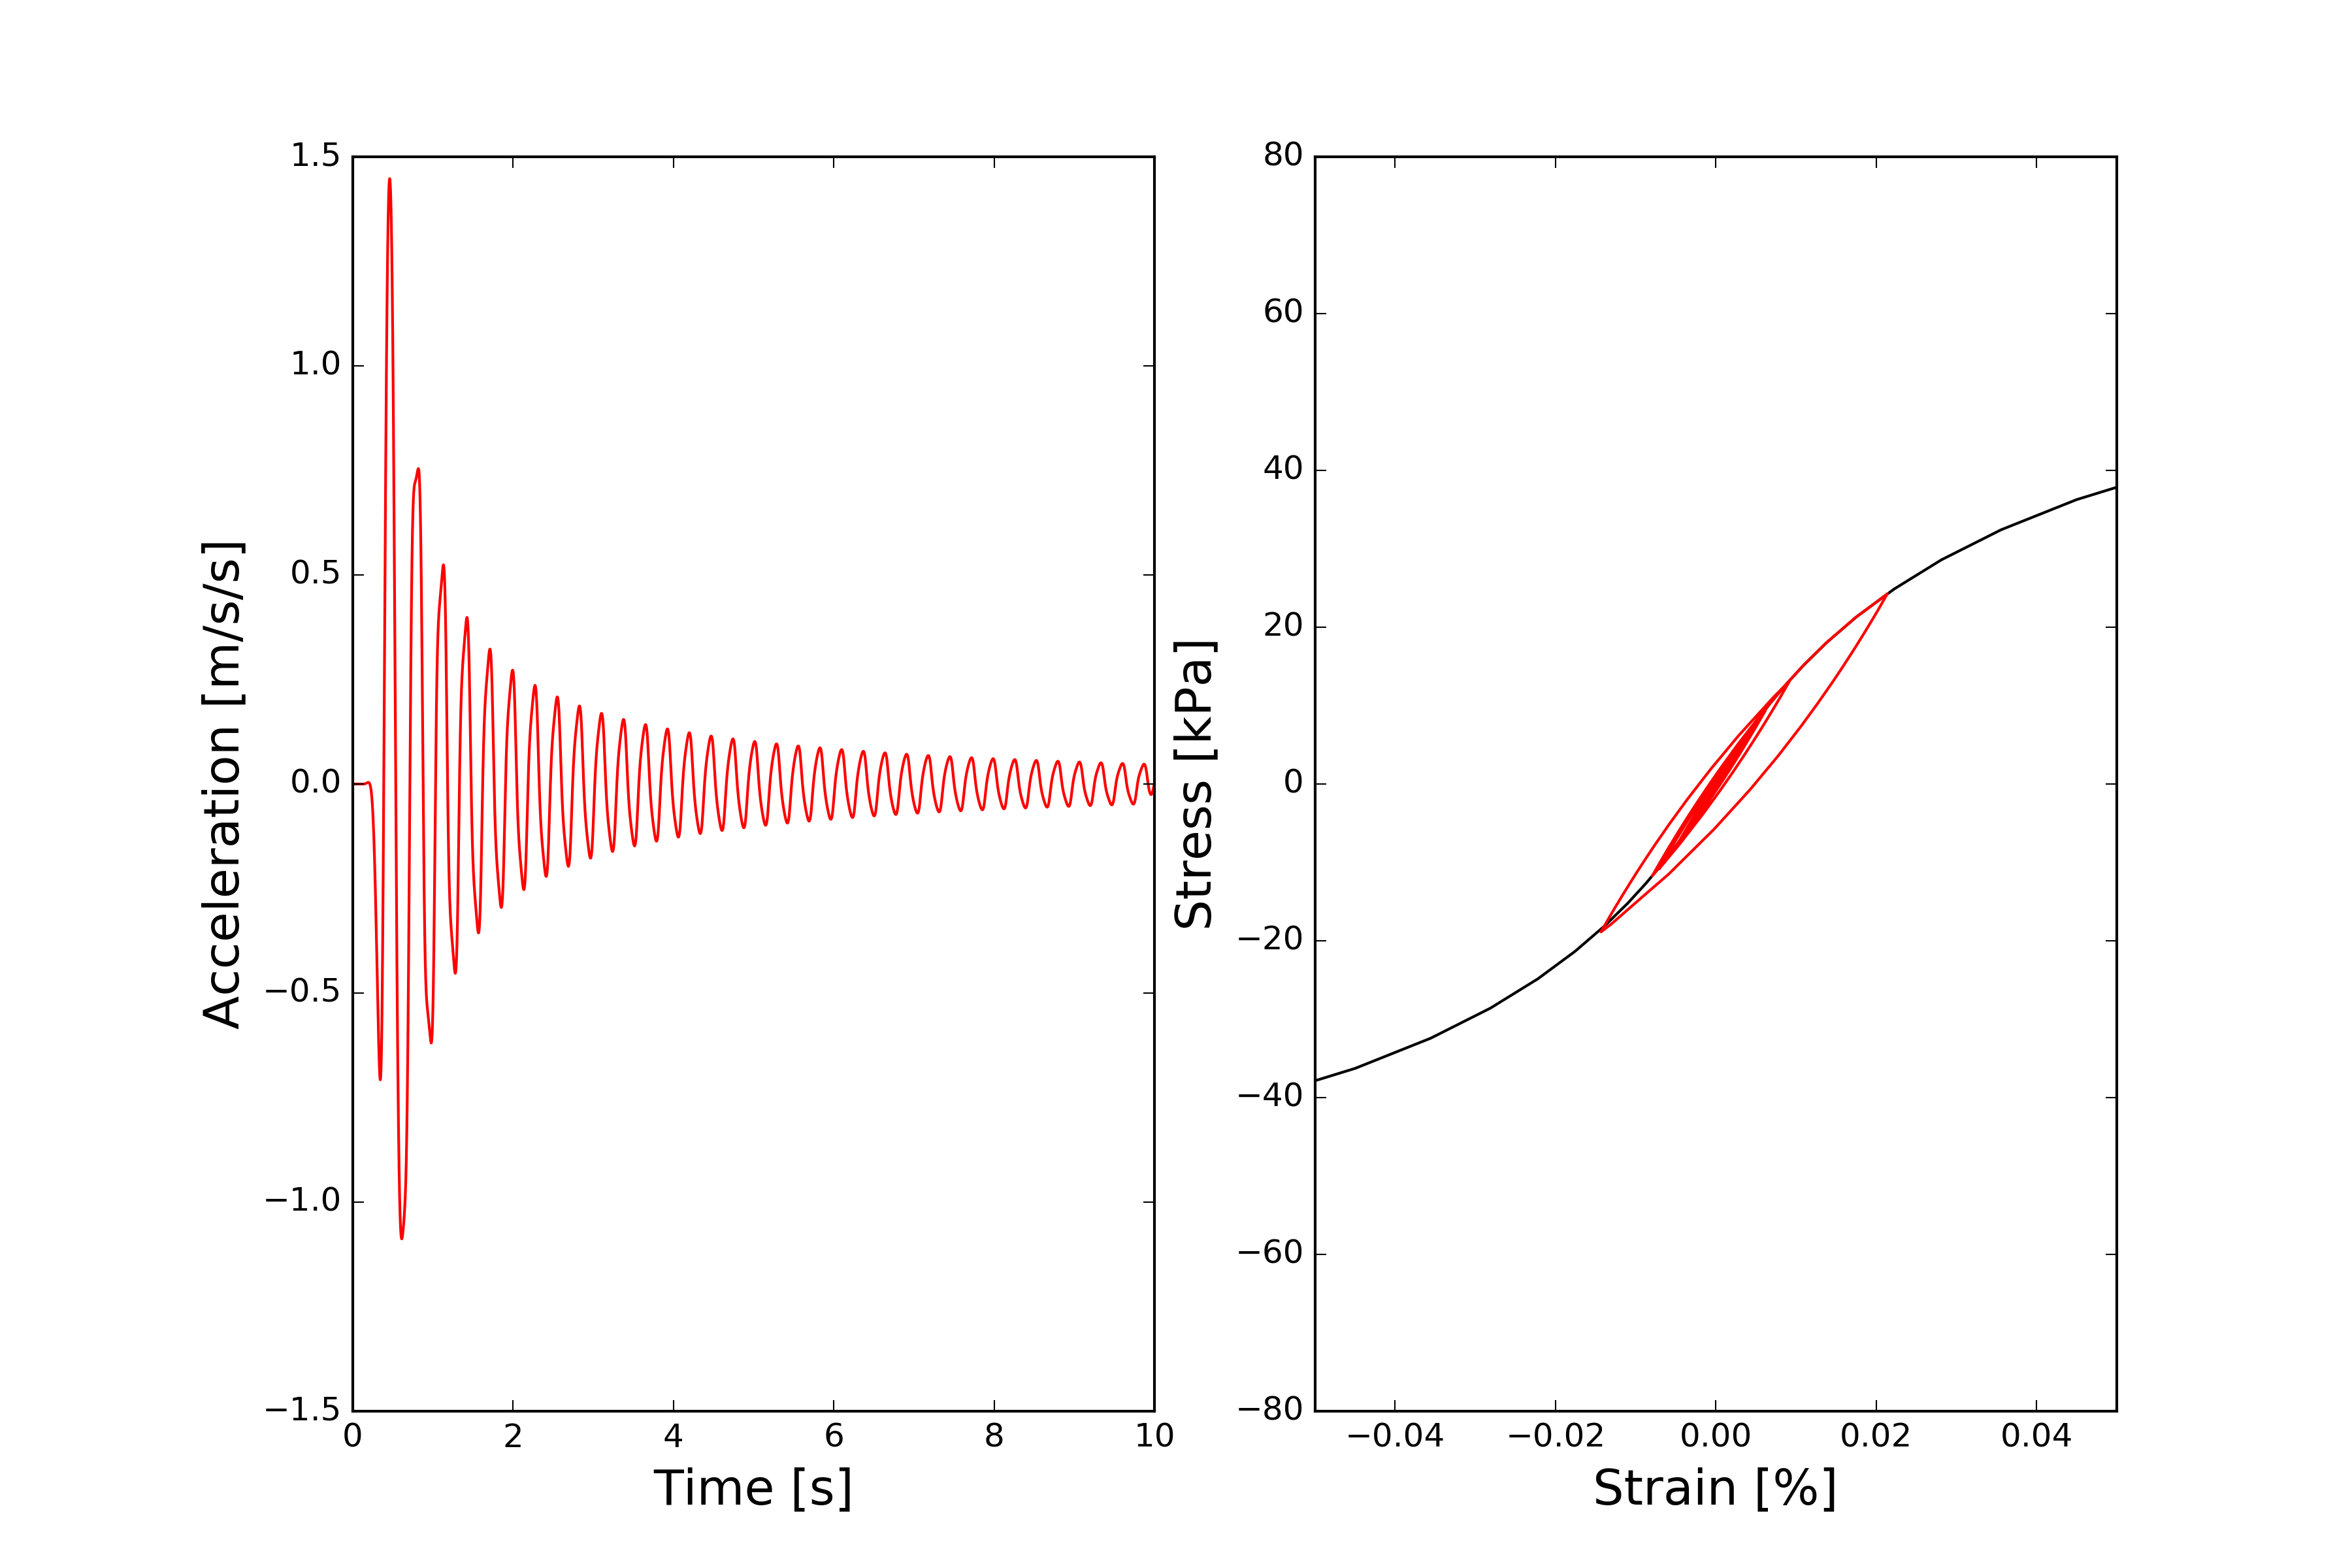
\includegraphics[scale=0.5]{figures/plot.eps} 
\captionof{figure}{Acceleration time histories at surface (left); Stress-strain curve at mid-column of P1 model (right).}
\label{plot} 
\vspace{1cm}
\end{center}



For plotting Fast Fourier transforms of a given file (acceleration or velocity time histories), fft.py file could be used. Resultant figure for WRLA model effective stress analysis is displayed in Figure \ref{fft}. \\


%% FIGURE : fft.png
\begin{center}
\leavevmode
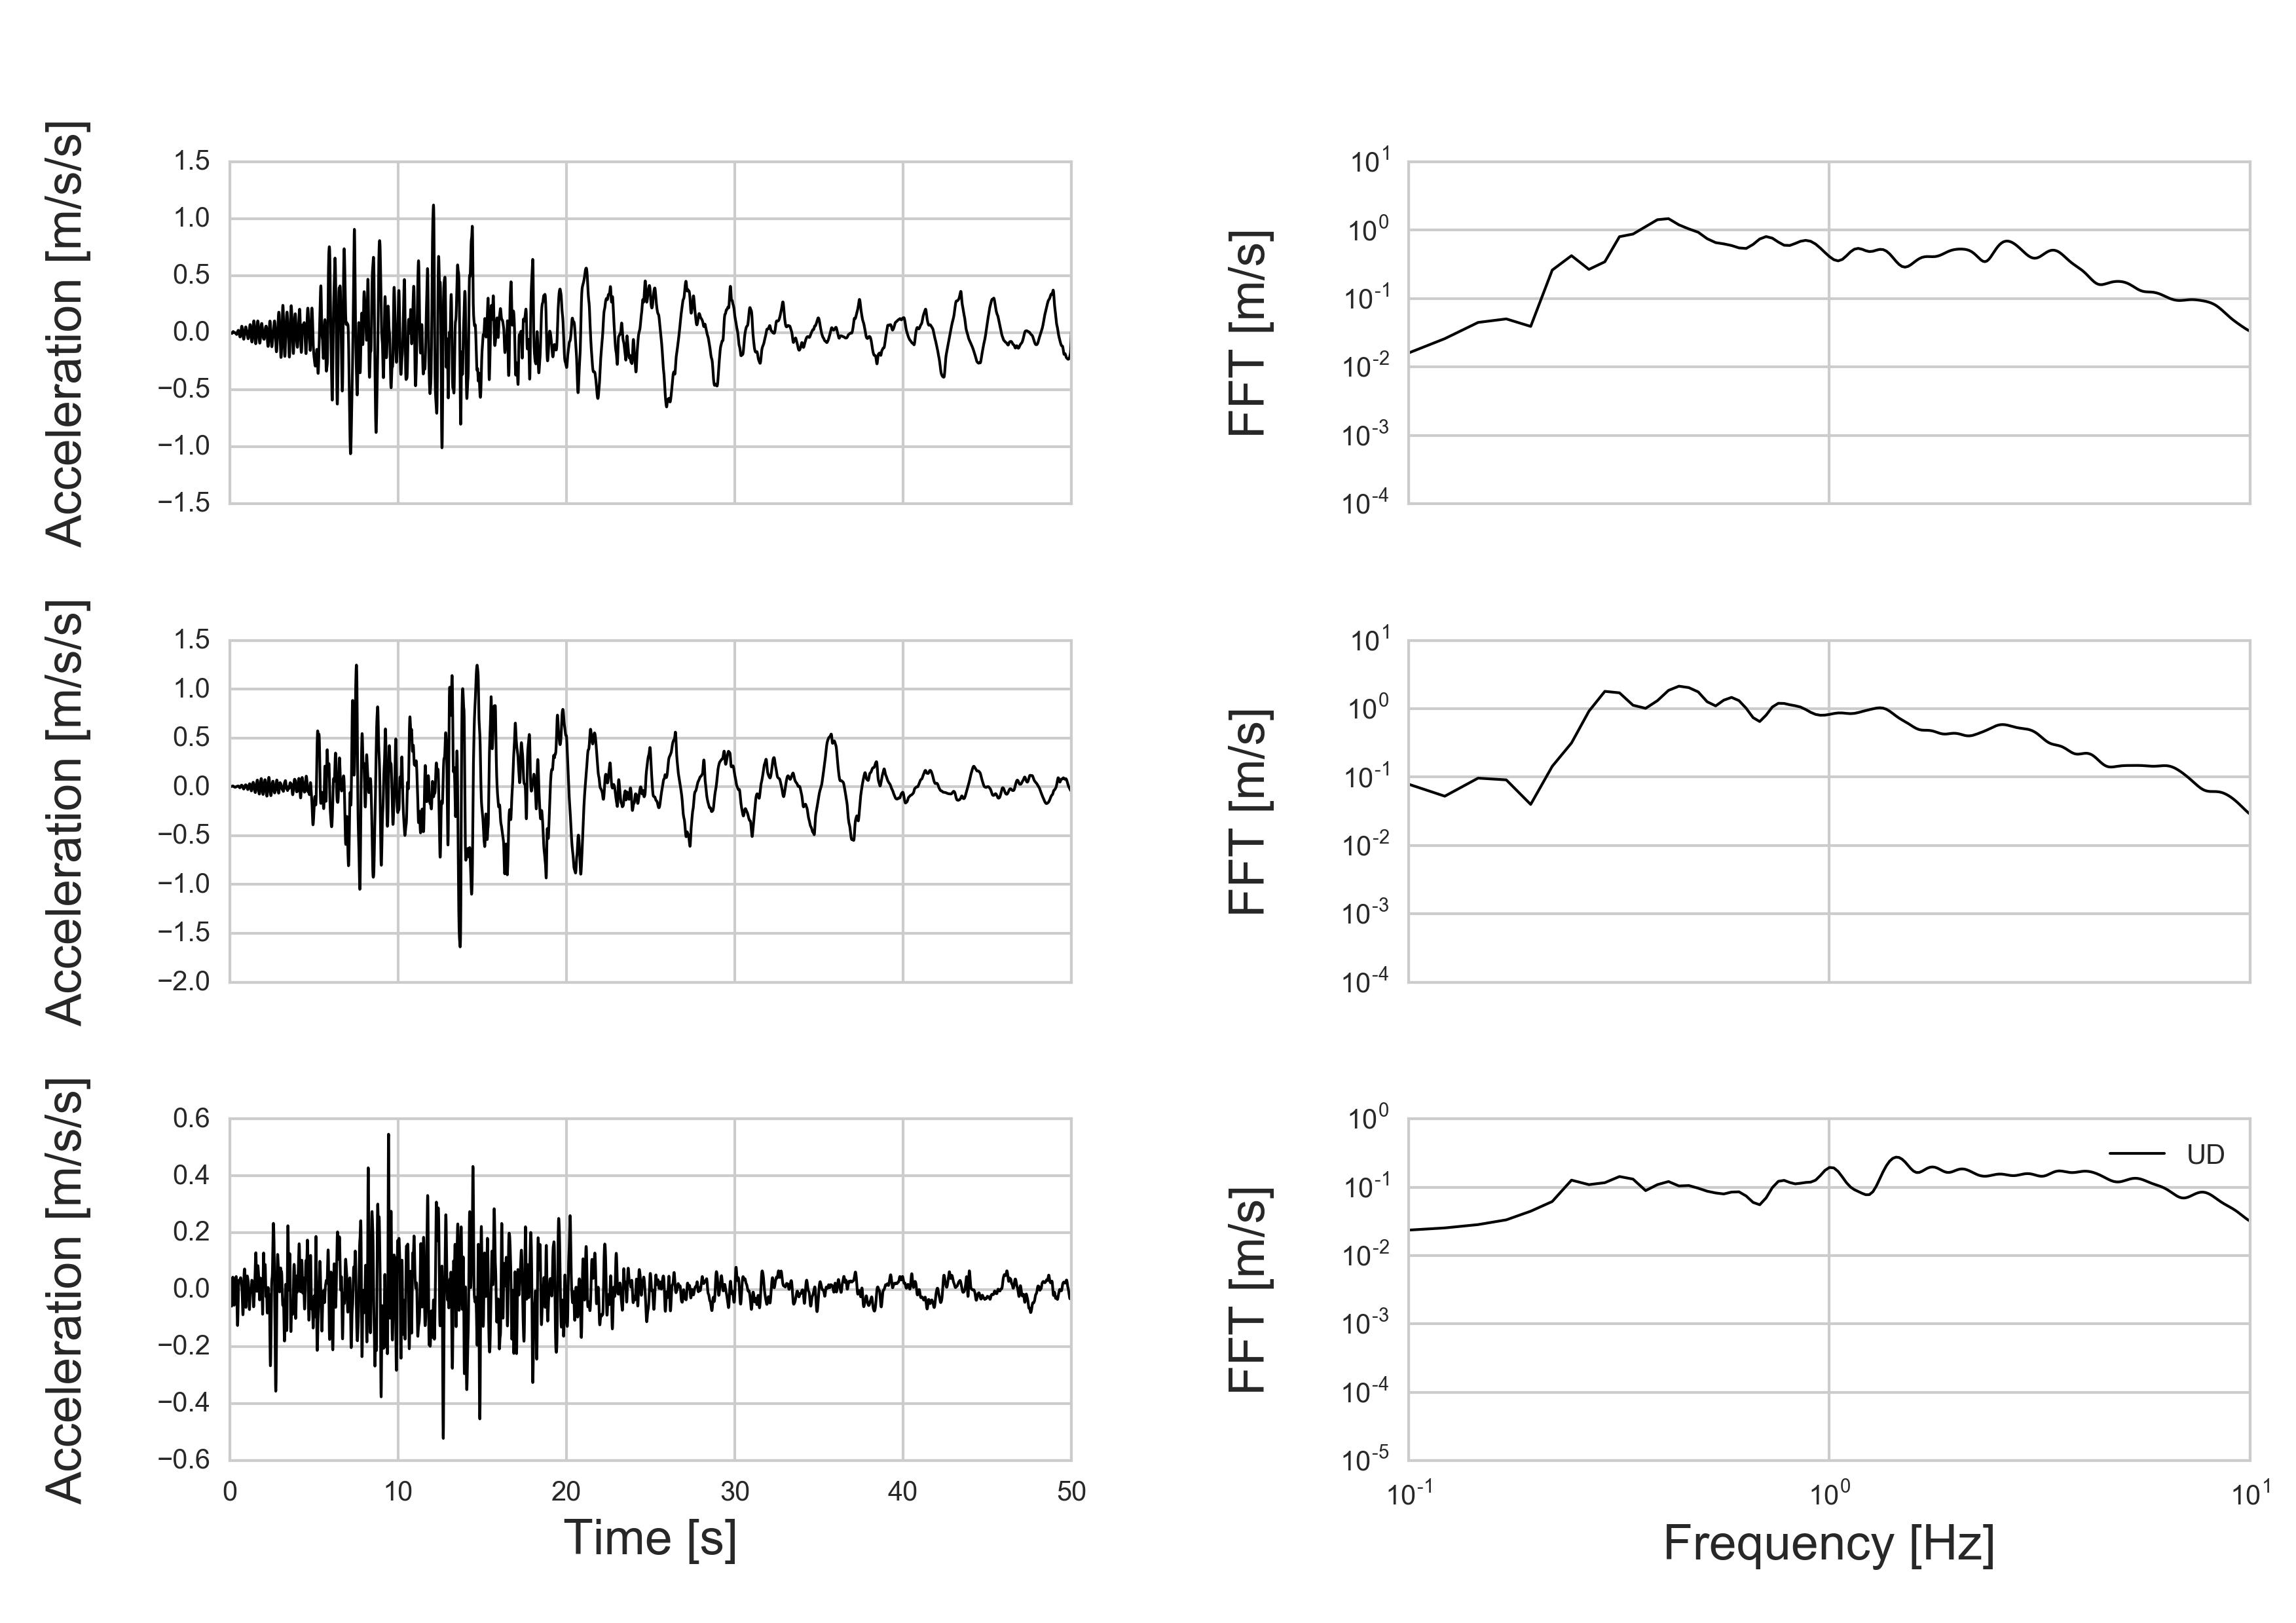
\includegraphics[scale=0.5]{figures/WRLA_acceleration_fft.eps} 
\captionof{figure}{Acceleration time histories at surface (left); Fast Fourier transform (right) for three directions of WRLA model effective stress analysis.}
\label{fft} 
\vspace{1cm}
\end{center}


For effective stress analyses, in order to visualize the changes in pore pressure excess, deviatoric plan, shear modulus and stress-strain curves, ‘effective\textunderscore changes.py’ file is ready to use. An example for WRLA model is shown in Figure \ref{eff}. \\


%% FIGURE : effective
\begin{center}
\leavevmode
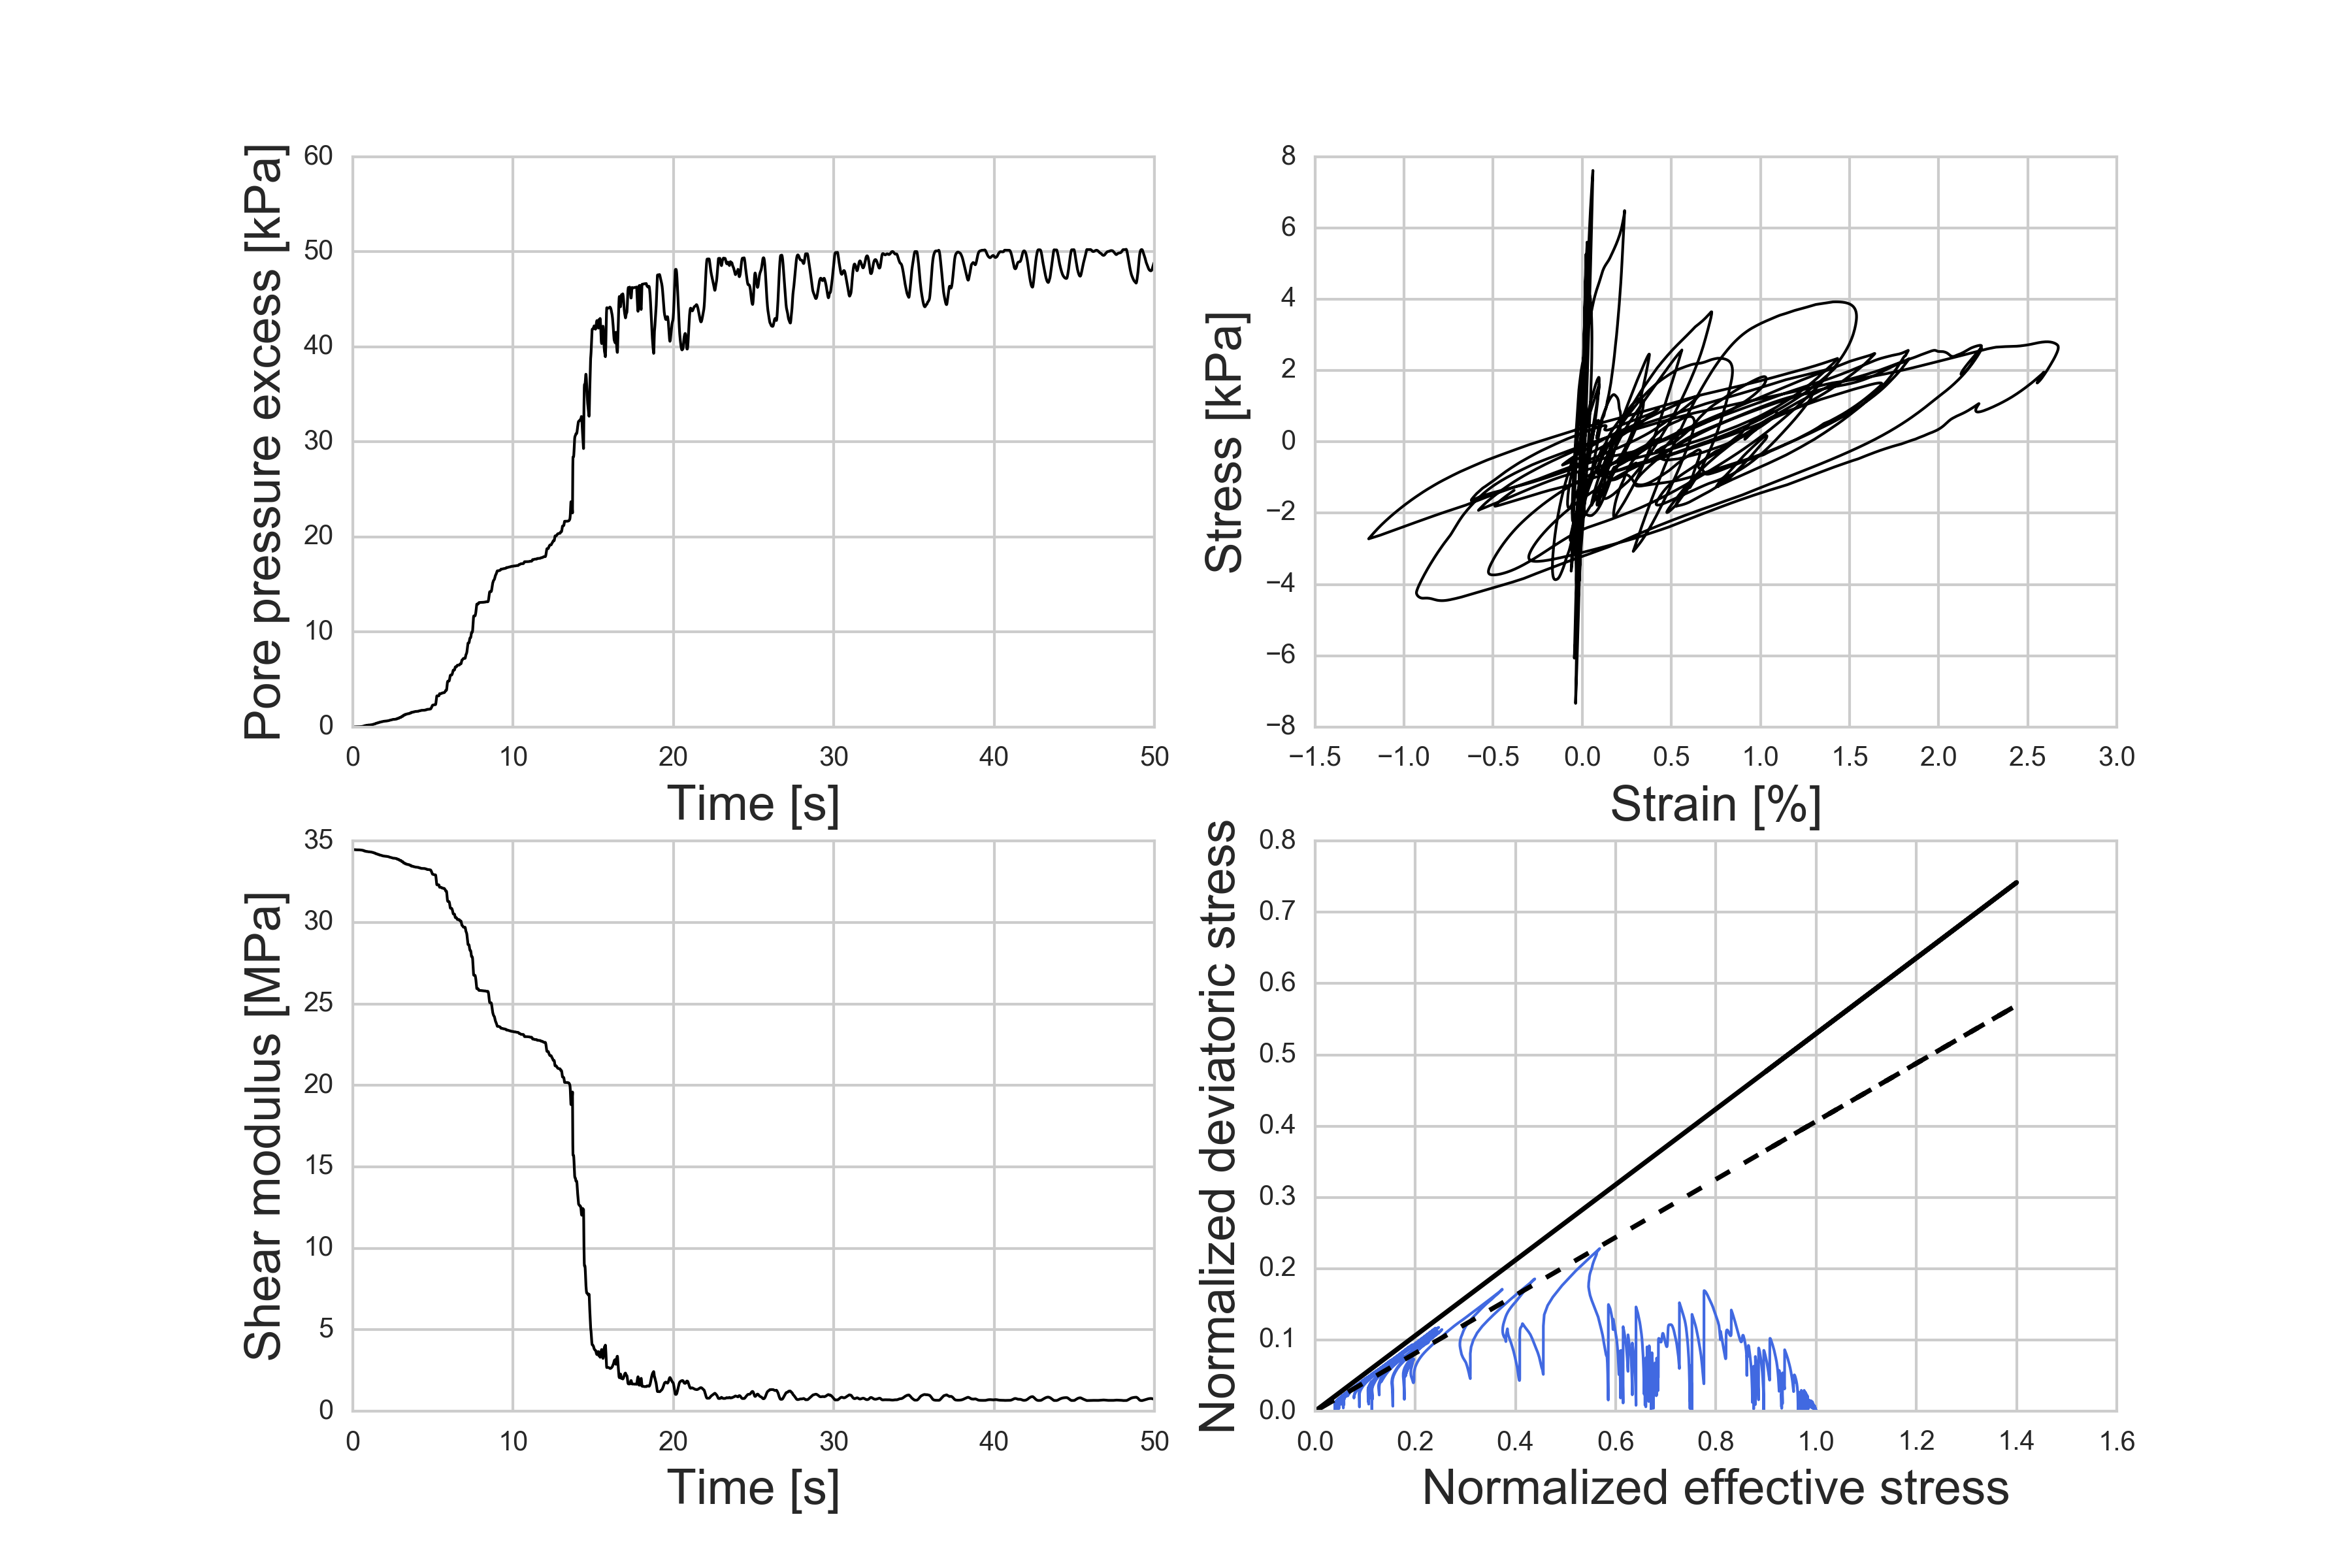
\includegraphics[scale=0.5]{figures/effective_stress_analysis.eps} 
\captionof{figure}{Pore pressure excess temporal change (left top); Stress-strain curve for EW-UD direction (top right); Change in shear modulus (bottom left); Deviatoric plan (bottom right) at GL-4 m for WRLA model effective stress analysis.}
\label{eff} 
\vspace{1cm}
\end{center}




